This study was conducted to test the viability of the DPGP tool on longitudinal RNA-seq data, with the end goal of including it in the project pipeline whether it produces reasonably sound results. For this purpose, DPGP was first used to recreate the findings published in its original paper \citep{mcdowellClusteringGeneExpression2018}, and then tested it on simulated datasets, as a way to assess its behaviour in a controlled setting environment with known expectations.

\section{Reproducing DPGP results}\label{res:geo}
The objective of this study was to obtain a result that is as close as possible to the analysis done by \citeauthor{mcdowellClusteringGeneExpression2018} in the DPGP paper, by focusing on the dataset obtained from the treatment of \textit{Halobacterium salinarum} with H\textsubscript{2}O\textsubscript{2}. Figure \ref{img:paper} -- which is labelled \emph{Fig 2} in the original paper -- shows the plots that were recreated in this study.

\begin{figure}[!ht]
    \centering
    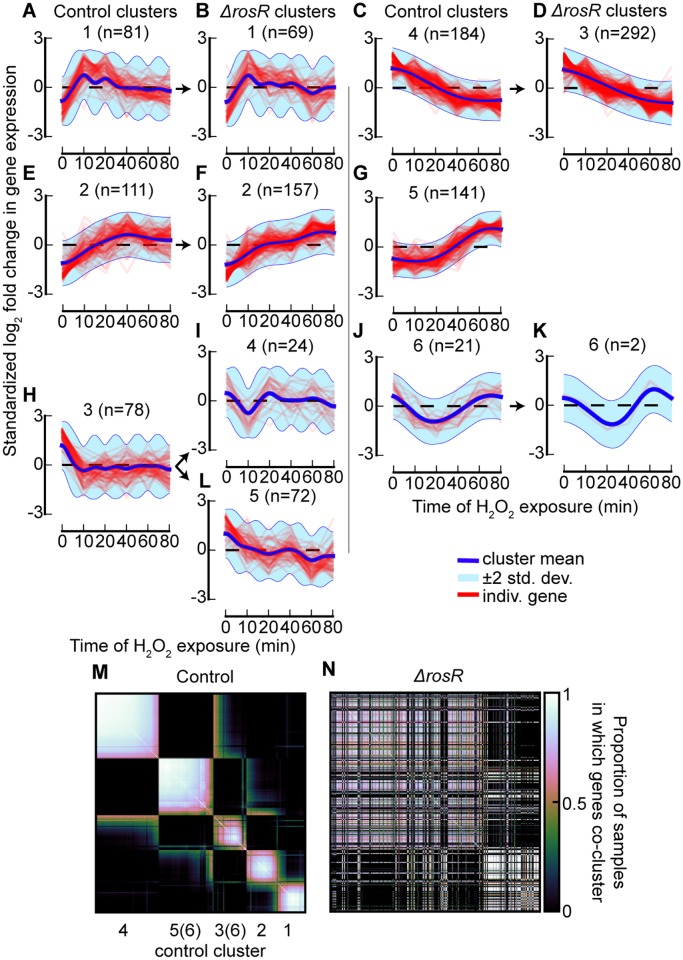
\includegraphics[width=.65\textwidth]{../DPGP/papers/pcbi.1005896.g002.jpg}
    \caption[Oxidative stress response clusters from \citeauthor{mcdowellClusteringGeneExpression2018}]{Original figure of the oxidative stress response clusters from \citealp{mcdowellClusteringGeneExpression2018}. (A-L) Gene expression trajectories for each cluster. Red lines are standardized $\log_{2}$ fold change of single gene expression. Blue lines are the posterior cluster mean expression levels. The first and third columns (panels A, E, H, C, G, and J) show control clusters, and the second and fourth columns (panels B, F, I, L, D, and K) the mutant clusters. The arrows point at the equivalent mutant cluster based on the Pearson correlation coefficient of the mean trajectories. (M, N) Heatmaps showing the proportion of sampled genes that cluster with every other gene for the control strain (M), and for the mutant $\Delta$rosR strain (N). The gene order has been determined by Ward's linkage for the control, and for the mutant it has been assigned the same order as the control.}\label{img:paper}
\end{figure}

First, the \href{https://www.ncbi.nlm.nih.gov/geo/query/acc.cgi?acc=GSE33980}{GEO GSE33980 dataset} was downloaded, which also contains data from a second experiment where \textit{H. salinarum} has been treated with a different compound. The pre-processing step filters that data out and prepares the expression matrices to input into DPGP (for the full description, see \ref{preprocess}). In the original work that produced the GEO dataset \citep{sharmaRosRTranscriptionFactor2012}, the authors identified 616 differentially expressed genes (DEGs) which they clustered using a k-means algorithm. \citeauthor{mcdowellClusteringGeneExpression2018} ran DPGP only on the DEGs and not the whole dataset, but it was not shared among the supplementary material of the DPGP paper, so the list of DEGs was retrieved from the supplementary material of the paper by \citeauthor{sharmaRosRTranscriptionFactor2012}. That table includes another version of the gene expression dataset already divided by experiment, so throughout the pre-processing step the same actions were performed on both datasets --  the one obtained from the supplementary material, and the one downloaded from the GEO database. After the individual expression matrices were obtained to be used as DPGP input, a comparison was performed using \texttt{diff}, which showed that the matching expression table files were identical (data not shown) therefore, throughout the analysis, only the dataset downloaded from the GEO database was used, because it is easier to access and publicly available, despite needing an extra filtering step.

\begin{figure}[!ht]
    \centering
    \parbox{.5\textwidth}{
        \textbf{a}\\
        \includegraphics[width=.5\textwidth]{../DPGP/results/GSE33980/paper/geo_ura3_gene_expression_fig_1.png}
    }
    \parbox{.45\textwidth}{
        \textbf{b}\\
        \includegraphics[width=.45\textwidth]{../DPGP/results/GSE33980/paper/geo_ura3_posterior_similarity_matrix_heatmap.png}
    }
    \caption[DPGP default output for the control strain]{DPGP default graphical output for the control strain. (a) Gene expression trajectories for each cluster. Red lines are standardized $\log_{2}$ fold change of single gene expression. Blue lines are the posterior cluster mean expression levels. (b) Heatmap showing the proportion of sampled genes that cluster with every other gene. The gene order has been determined by complete linkage (using the \texttt{linkage} function within \texttt{SciPy}), and displayed as a dendrogram on the left.}\label{img:dpgp_ctrl}
\end{figure}

Then, by running the script \texttt{dpgp\_gse33980\_paper.sh}, DPGP is iteratively executed for both strains. The same flags and parameters used by \citeauthor{mcdowellClusteringGeneExpression2018} were used, even though some of their choices could be disputed. For instance, they claimed that the fast (fDPGP) and default implementation of DPGP gave very similar results on simulated datasets, so they chose to use fDPGP for all biological data. However, when the default DPGP was run on the same GEO dataset, the results were very different: 17 clusters for the control strain, with median 34 genes per cluster, and 14 clusters for the mutant strain, with median 27 genes per cluster (data not shown). They also used a lower value for the \emph{shape} hyperparameter, which is done to allow for a greater marginal variance within clusters. This is the case of microarray data, but they did not specify how they chose a particular shape value, making it a quite arbitrary choice. Lastly, the tool has an argument that allows for the true time difference between time point to be modelled, but the authors did not pass it, so the model assumed that all the time points are equally spaced, which means that the rate of change in expression is roughly equivalent between all neighbouring time points. Conceptually speaking, this may be true depending on the time course of the experiment but, in this case, it could have affected the analysis, because the first three time points are \SI{10}{\min} apart, and the next three are \SI{20}{\min} apart. In an organism like \textit{H. salinarum} -- or in a model bacterium -- this can be equivalent to twice the number of replication cycles, and significant changes in gene expression.

Nevertheless, with the parameters used by \citeauthor{mcdowellClusteringGeneExpression2018}, the results were almost identical to the ones shown in the paper. Figures \ref{img:dpgp_ctrl} and \ref{img:dpgp_mut} show the default DPGP graphical output, corresponding to the gene expression trajectories of all the clusters (panel a), and to the heatmap of the proportion of sampled genes that cluster together (panel b). The latter may be used to visualize at a glance the main groups within the data, identified by the genes that more consistently are clustered together are closer to the diagonal and forms whiter squares, or by genes that are represented by other hues and are farther from the diagonal have a chance to be clustered in other cluster. The main white ``blocks'' are indicative of the main clusters.

\begin{figure}[!ht]
    \centering
    \parbox{.5\textwidth}{
        \textbf{a}\\
        \includegraphics[width=.5\textwidth]{../DPGP/results/GSE33980/paper/geo_d258_gene_expression_fig_1.png}
    }
    \parbox{.45\textwidth}{
        \textbf{b}\\
        \includegraphics[width=.45\textwidth]{../DPGP/results/GSE33980/paper/geo_d258_posterior_similarity_matrix_heatmap.png}
    }
    \caption[DPGP default output for the mutant strain]{DPGP default graphical output for the mutant strain. (a) Gene expression trajectories for each cluster. Red lines are standardized $\log_{2}$ fold change of single gene expression. Blue lines are the posterior cluster mean expression levels. (b) Heatmap showing the proportion of sampled genes that cluster with every other gene. The gene order has been determined by complete linkage (using the \texttt{linkage} function within \texttt{SciPy}), and displayed as a dendrogram on the left.}\label{img:dpgp_mut}
\end{figure}

Figure \ref{img:dpgp_mut} shows the default graphical output for the mutant strain. When compared to the corresponding graphs in figure \ref{img:paper}, both the gene expression trajectories and the number of genes in each cluster are identical. The heatmaps (figure \ref{img:dpgp_mut} panel b and figure \ref{img:paper} panel N) are different because the one in the paper was obtained by rearranging the order of the genes. The output for the control strain (figure \ref{img:dpgp_ctrl}) is instead slightly different from the corresponding published one, in terms of gene trajectories, number of gene assignment, and heatmap visualization. This can be explained by two possible scenarios: either the authors used a different seed when clustering the mutant strain, or they processed those data in a way not accounted in this study without documenting it.

\subsection{Equivalent clusters}\label{eq_clust}
In order to identify corresponding equivalent cluster pairs, functions present in the code of DPGP software was adapted to export the posterior cluster mean expression trajectories (represented by the blue lines), since the standard output does not include them. Then, the Pearson correlation coefficient between all possible mean trajectory pairs was calculated. The resulting $r$ values are collected in table \ref{tab:pearson}.

\begin{table}[!ht]
    \centering\footnotesize
    \begin{tabular}{l|rrrrrr}
 & mut cluster 1 & mut cluster 2 & mut cluster 3 & mut cluster 4 & mut cluster 5 & mut cluster 6 \\
\hline
ctrl cluster 1 & \cellcolor{lightgray} \bfseries 0.8867 & -0.0080 & 0.1128 & -0.3315 & -0.1528 & -0.6432 \\
ctrl cluster 2 & 0.2599 & \cellcolor{lightgray} \bfseries 0.7708 & -0.7663 & 0.2601 & -0.7118 & -0.3161 \\
ctrl cluster 3 & -0.7122 & -0.6457 & 0.5704 & 0.1651 & \cellcolor{lightgray} \bfseries 0.7097 & 0.4704 \\
ctrl cluster 4 & 0.0866 & -0.9131 & \cellcolor{lightgray} \bfseries 0.9338 & -0.1773 & 0.8104 & -0.1514 \\
ctrl cluster 5 & -0.4718 & \cellcolor{lightgray} \bfseries 0.7939 & -0.8350 & 0.0442 & -0.6852 & 0.6682 \\
ctrl cluster 6 & -0.8280 & 0.0777 & -0.1538 & 0.0047 & 0.0398 & \cellcolor{lightgray} \bfseries 0.8915 \\
\end{tabular}

    \caption[Clusters pairwise Pearson correlation coefficient]{Pearson correlation coefficient between all possible pairs of posterior cluster mean expression level. Clusters obtained from the control strain are represented as rows, and clusters obtained from the mutant strain are represented as columns. Highlighted values are the highest values from a column-wise comparison, which correspond to the cluster pair with the most similar mean expression trajectory.}\label{tab:pearson}
\end{table}

By performing a column-wise comparison, the cluster pairs with the highest Pearson correlation coefficient (highlighted values) were selected, and each pair was plotted with the control and mutant clusters side by side, mirroring the pairing done by \citeauthor{mcdowellClusteringGeneExpression2018} in figure \ref{img:paper} with the pointing arrows. 

\begin{figure}[!ht]
    \centering
    \parbox{.4\textwidth}{
        \textbf{a}\\
        \includegraphics[width=.4\textwidth]{../DPGP/results/GSE33980/paper/geo_ura3_fig_1.png}
    }
    \parbox{.4\textwidth}{
        \textbf{b}\\
        \includegraphics[width=.4\textwidth]{../DPGP/results/GSE33980/paper/geo_d258_fig_1.png}
    }
    \caption[Equivalent cluster 1 pair]{Equivalent cluster pair: control cluster 1 (a) and mutant cluster 1 (b). Red lines are standardized $\log_{2}$ fold change of single gene expression trajectories. Blue lines are the posterior cluster mean expression levels.}\label{img:clust1}
\end{figure}

\begin{figure}[!ht]
    \centering
    \parbox{.4\textwidth}{
        \textbf{a}\\
        \includegraphics[width=.4\textwidth]{../DPGP/results/GSE33980/paper/geo_ura3_fig_2.png}
    }
    \parbox{.4\textwidth}{
        \textbf{b}\\
        \includegraphics[width=.4\textwidth]{../DPGP/results/GSE33980/paper/geo_d258_fig_2.png}
    }
    \caption[Equivalent cluster 2 pair]{Equivalent cluster pair: control cluster 2 (a) and mutant cluster 2 (b). Red lines are standardized $\log_{2}$ fold change of single gene expression trajectories. Blue lines are the posterior cluster mean expression levels.}\label{img:clust2}
\end{figure}

Figures \ref{img:clust1} and \ref{img:clust2} show a very consistent pairing to the one in the paper ($r=\num{0.8867}$, $p=\num{5.35e-169}$, and $r=\num{0.7708}$, $p=\num{1.38e-99}$ respectively), with a fast spike in expression levels followed by downregulation to base level for the cluster 1 pair, and a somewhat steady upregulation for the cluster 2 pair.

\begin{figure}[!ht]
    \centering
    \parbox{.4\textwidth}{
        \textbf{a}\\
        \includegraphics[width=.4\textwidth]{../DPGP/results/GSE33980/paper/geo_ura3_fig_3.png}
    }
    \parbox{.4\textwidth}{
        \textbf{b}\\
        \includegraphics[width=.4\textwidth]{../DPGP/results/GSE33980/paper/geo_d258_fig_5.png}
    }
    \caption[Equivalent cluster 3 pair]{Equivalent cluster pair: control cluster 3 (a) and mutant cluster 5 (b). Red lines are standardized $\log_{2}$ fold change of single gene expression trajectories. Blue lines are the posterior cluster mean expression levels.}\label{img:clust3}
\end{figure}

Figure \ref{img:clust3} starts to diverge from the analysis in the paper, because mutant cluster 5 was also identified as the equivalent one ($r=\num{0.7097}$, $p=\num{8.57e-78}$), but mutant cluster 4 could not since it does not have even the second-highest Pearson correlation coefficient ($r=\num{0.1651}$), unlike what \citeauthor{mcdowellClusteringGeneExpression2018} reported (see figure \ref{img:paper} panels H, I, and L).

\begin{figure}[!ht]
    \centering
    \parbox{.4\textwidth}{
        \textbf{a}\\
        \includegraphics[width=.4\textwidth]{../DPGP/results/GSE33980/paper/geo_ura3_fig_4.png}
    }
    \parbox{.4\textwidth}{
        \textbf{b}\\
        \includegraphics[width=.4\textwidth]{../DPGP/results/GSE33980/paper/geo_d258_fig_3.png}
    }
    \caption[Equivalent cluster 4 pair]{Equivalent cluster pair: control cluster 4 (a) and mutant cluster 3 (b). Red lines are standardized $\log_{2}$ fold change of single gene expression trajectories. Blue lines are the posterior cluster mean expression levels.}\label{img:clust4}
\end{figure}

Figure \ref{img:clust4} has the highest correlation of all pairings ($r=\num{0.9338}$, $p=\num{1.91e-224}$), showing a steady downregulation trajectory over time.

\begin{figure}[!ht]
    \centering
    \parbox{.4\textwidth}{
        \textbf{a}\\
        \includegraphics[width=.4\textwidth]{../DPGP/results/GSE33980/paper/geo_ura3_fig_5.png}
    }
    \parbox{.4\textwidth}{
        \textbf{b}\\
        \includegraphics[width=.4\textwidth]{../DPGP/results/GSE33980/paper/geo_d258_fig_2.png}
    }
    \caption[Equivalent cluster 5 pair]{Equivalent cluster pair: control cluster 5 (a) and mutant cluster 2 (b). Red lines are standardized $\log_{2}$ fold change of single gene expression trajectories. Blue lines are the posterior cluster mean expression levels.}\label{img:clust5}
\end{figure}

Figure \ref{img:clust5} shows the most inconsistent pairing compared to the published one. \citeauthor{mcdowellClusteringGeneExpression2018} reported that control cluster 5 does not have an equivalent cluster among the mutant ones, but there are clusters with a clear similar trajectory. Moreover, the way they evaluated this equivalence is by computing the Pearson correlation coefficient and selecting the highest one among a series of possible pairs; even in the case all $r$ values were very low, or even close to -1 (denoting a complete opposite behaviour), by selecting the highest value they could still get the closest possible expression trajectory. For these reasons, the pairing shown in figure \ref{img:clust5} is reasonable, as also proven by the statistic ($r=\num{0.7939}$, $p=\num{1.17e-109}$), which is not even the lowest among all equivalent pairs.

\begin{figure}[!ht]
    \centering
    \parbox{.4\textwidth}{
        \textbf{a}\\
        \includegraphics[width=.4\textwidth]{../DPGP/results/GSE33980/paper/geo_ura3_fig_6.png}
    }
    \parbox{.4\textwidth}{
        \textbf{b}\\
        \includegraphics[width=.4\textwidth]{../DPGP/results/GSE33980/paper/geo_d258_fig_6.png}
    }
    \caption[Equivalent cluster 6 pair]{Equivalent cluster pair: control cluster 6 (a) and mutant cluster 6 (b). Red lines are standardized $\log_{2}$ fold change of single gene expression trajectories. Blue lines are the posterior cluster mean expression levels.}\label{img:clust6}
\end{figure}

Lastly, figure \ref{img:clust6} shows another quite consistent pairing ($r=\num{0.8915}$, $p=\num{2.33e-173}$), characterized by a dip in expression levels towards the middle time points, returning to baseline levels at later stages. Despite this observation, the very low number of genes assigned to these clusters makes them poorly represented clusters that may not correspond to true groups in the dataset. In fact, the two heatmaps -- figure \ref{img:dpgp_ctrl}.b for the control, and figure \ref{img:dpgp_mut}.b for the mutant -- show 5 and 3 major groups respectively.

% \clearpage
\subsection{Cluster switching}
\citeauthor{mcdowellClusteringGeneExpression2018} then proceeded with the testing of the statistical significance of cluster switching among genes, by calculating the Fisher's exact test. To do so, the number of genes that belong to all possible cluster pairing was computed by looking at the intersection of the list of gene labels in each control cluster \textit{vs.} each mutant one. Table \ref{tab:cocluster} is the resulting count table, where the highlighted cells correspond to the equivalent gene trajectory behaviour as assessed in section \ref{eq_clust}.

\begin{table}[!ht]
    \centering\footnotesize
    \begin{tabular}{l|rrrrrr}
 & mut cluster 1 & mut cluster 2 & mut cluster 3 & mut cluster 4 & mut cluster 5 & mut cluster 6 \\
\hline
ctrl cluster 1 & \cellcolor{lightgray} \bfseries 30 & 44 & 7 & 1 & 1 & 0 \\
ctrl cluster 2 & 11 & \cellcolor{lightgray} \bfseries 64 & 12 & 2 & 3 & 1 \\
ctrl cluster 3 & 0 & 3 & 56 & 8 & \cellcolor{lightgray} \bfseries 18 & 0 \\
ctrl cluster 4 & 11 & 10 & \cellcolor{lightgray} \bfseries 125 & 3 & 29 & 0 \\
ctrl cluster 5 & 17 & \cellcolor{lightgray} \bfseries 35 & 78 & 8 & 16 & 1 \\
ctrl cluster 6 & 0 & 1 & 14 & 2 & 5 & \cellcolor{lightgray} \bfseries 0 \\
\end{tabular}

    \caption[Co-clustered genes in each pairwise combination]{Number of genes belonging to both control and mutant clusters. Each value represents the same list of genes that are assigned to that particular cluster pair. This basically is a contingency table of all control clusters \textit{vs.} all mutant clusters. Highlighted values correspond to the number of genes that are clustered in the equivalent mutant strain cluster (as identified by Pearson correlation, see \ref{tab:pearson}), meaning that they maintain the same expression behaviour over time.}\label{tab:cocluster}
\end{table}

It is worth mentioning that the number of genes that belong to a clusters pair is not taken into account for the ``equivalence'' assessment -- only the mean expression levels are. In fact, clusters can be considered as ``behaviours'' of the genes, which are represented as trajectories of expression levels over time (\textit{e.g.} initial upregulation followed by stationary expression, or upregulation followed by downregulation, or downregulation at later time, and so on).
For instance, the equivalent pair for cluster 6 does not contain any gene, meaning that all those genes displayed a different behaviour if they came from the control or the mutant strain. In this particular case, \citeauthor{mcdowellClusteringGeneExpression2018} would not have considered this pair as equivalent clusters (joined by an arrow) because they had no co-clustered genes -- analogously to what they claimed for control cluster 5 -- but, by considering clusters as model behaviours, it is logical to assign to each cluster its equivalent. Moreover, a 2 by 2 contingency table has to be generated in order to compute the Fisher's exact test, so there have to be two categorical variables to count, in this case belonging to the control cluster \textit{vs.} to the mutant cluster in each pair of clusters.  

For each of the equivalent cluster pair, table \ref{tab:cocluster} was used to calculate a contingency table, which I then used to compute the Fisher's exact test. Because the \texttt{fisher\_exact} function within the same \texttt{SciPy} module was used, the statistic produced is not the same as the standard function implemented in R: the \texttt{SciPy} function calculates the odds ratio, and the R function the conditional maximum likelihood estimate.

A final summary table \ref{tab:eq_clust} recapitulates the statistical analysis on the equivalent gene trajectory pairs. By taking into account the number of genes that get assigned to each cluster, the first four pairings have a statistically significant relationship, but cluster switching for the control cluster 5 pair is not significant, as opposed to what reported in the paper ($p \leq \num{2.2e-16}$). The number of genes that display a different dynamic was also reported -- meaning they belong to any other cluster except the one deemed equivalent -- because \citeauthor{mcdowellClusteringGeneExpression2018} used the number of total genes with different dynamic to compare their results with the ones previously published by \citeauthor{sharmaRosRTranscriptionFactor2012}. In this regard, the results in this study are reasonably similar to the one published, despite the discrepancies discussed so far: the total number of genes that show a different expression trajectory in the mutant strain group is 344, \textit{vs.} 372 reported in the paper.

\begin{table}[!ht]
    \centering\footnotesize
    \begin{tabular}{>{\centering}m{1.7cm}>{\centering}m{1.8cm}>{\centering}m{1.2cm}S[table-format = 1.2e2]>{\centering}m{1cm}S[table-format = 1.2e2]>{\centering}m{2.2cm}p{0pt}}
\textbf{Control strain} & \textbf{Mutant strain} & \textbf{Pearson corr r} & \textbf{Pearson p value} & \textbf{Odds ratio} & \textbf{FET p value} & \textbf{Different dynamic genes} & \textbf{} \\
ctrl cluster 1 & mut cluster 1 & 0.8867 & 5.35e-169 & 7.17 & 3.08e-11 &  53 (63.9\%) &  \\
ctrl cluster 2 & mut cluster 2 & 0.7708 & 1.38e-99 & 10.20 & 4.09e-22 &  29 (31.2\%) &  \\
ctrl cluster 3 & mut cluster 5 & 0.7097 & 8.57e-78 & 2.37 & 5.92e-03 &  67 (78.8\%) &  \\
ctrl cluster 4 & mut cluster 3 & 0.9338 & 1.91e-224 & 3.83 & 5.31e-13 &  53 (29.8\%) &  \\
ctrl cluster 5 & mut cluster 2 & 0.7939 & 1.17e-109 & 0.81 & 3.94e-01 & 120 (77.4\%) &  \\
ctrl cluster 6 & mut cluster 6 & 0.8915 & 2.33e-173 & 0.00 & 1.00e+00 &  22 (100.0\%) &  \\
\end{tabular}

    \caption[Equivalent cluster summary]{Summary of the statistical analysis of the equivalent cluster pairs. Pearson correlation $r$ and $p$ values are calculated with the \texttt{pearsonr} function of the Python \texttt{SciPy} module \citep{virtanenSciPyFundamentalAlgorithms2020}. Odds ratio and Fisher's exact test (FET) $p$ value are calculated using the \texttt{fisher\_exact} function within the same \texttt{SciPy} module. The number of genes with different dynamic is calculated using the relative contingency table, and expressed as a percentage of the total number of genes in that cluster.}\label{tab:eq_clust}
\end{table}

Although these results would suggest otherwise, control cluster 5 was examined more closely because the authors focused on it. Of the 155 genes belonging to it, 120 (77.4\%) exhibit a different dynamic in the mutant strain. Since this cluster has an up-regulated trajectory over time, the trajectory of genes that have an inverted dynamic -- downregulated trajectory -- was evaluated, restricting the previous 120 genes to 94 (60.7\%), of which 78 belonged to mutant cluster 3, and 16 to mutant cluster 5.
In the paper, the authors got very similar numbers: out of 141 genes in control cluster 5 (which all of them had different dynamic in the mutant strain), 89 (63.1\%) had an inverted dynamic in gene expression trajectory, of which 72 belonged to mutant cluster 3, and 17 to mutant cluster 5.

All together, these findings suggest that DPGP produces very consistent results, in line with previously published observations.

\subsection{Heatmaps}
To conclude the analysis, a Python script recreated the heatmaps as shown in the original paper, by adapting functions present in the DPGP code to produce the images without the dendrograms, and adding the possibility to change the order of the genes.

Figure \ref{img:heatmap} shows the resulting heatmaps for the control (panel a) and mutant (panel b) strains but, since the latter is not present in the original paper, only the former is taken into consideration. The control strain heatmap shows a slightly different proportion matrix, in particular in the ``perpendicular stripes'' regions that seem to be displaced because of a different order. Unfortunately, without the dendrogram or the list of genes produced by the linkage, it is not possible to assert this for certain. Another possibility is that DPGP may have been run using a different seed, hence the different results, which in turn would be reflected in the heatmap. Alternatively, it may also be due to the linkage algorithm: in the caption of the figure in the original paper, the authors state that they used Ward's linkage, but in the DPGP code, the function that produces the gene order performs a complete linkage, which is the one used in this study.

\begin{figure}[!ht]
    \centering
    \parbox{.45\textwidth}{
        \textbf{a}\\
        \includegraphics[width=.45\textwidth]{../DPGP/results/GSE33980/paper/geo_ura3_heatmap.png}
    }
    \parbox{.45\textwidth}{
        \textbf{b}\\
        \includegraphics[width=.45\textwidth]{../DPGP/results/GSE33980/paper/geo_d258_heatmap.png}
    }
    \caption[Heatmap comparison between control and mutant clusters]{Heatmaps for the control (a) and mutant (b) strains, showing the proportion of sampled genes that cluster with every other gene. The gene order has been determined by complete linkage (using the linkage function within SciPy).}\label{img:heatmap}
\end{figure}

Lastly, figure \ref{img:heatmap_alt} shows the heatmaps for the two strains, where the order of the genes is the same for both the control (panel a) and the mutant (panel b). Although the images match those from the original text, no conclusive interpretation could be made, other than the pattern disruption: had the genes kept the same gene expression trajectory in the mutant strain, they would have had similar sampled proportions, resulting in ``whiter blocks'' in the same positions. The fact that the patterns are completely disrupted but in very few and small sections, means that the two clustered strains have distinct gene groupings.

\begin{figure}[!ht]
    \centering
    \parbox{.45\textwidth}{
        \textbf{a}\\
        \includegraphics[width=.45\textwidth]{../DPGP/results/GSE33980/paper/geo_ura3_heatmap.png}
    }
    \parbox{.45\textwidth}{
        \textbf{b}\\
        \includegraphics[width=.45\textwidth]{../DPGP/results/GSE33980/paper/geo_d258_alt_heatmap.png}
    }
    \caption[Heatmap comparison with alternative order]{Heatmaps showing the proportion of sampled genes that cluster with every other gene. For the control strain (a), the gene order has been determined by complete linkage (using the linkage function within SciPy). For the mutant strain (b), it has been used the same gene order as the control strain.}\label{img:heatmap_alt}
\end{figure}

\section{Using DPGP on simulated data}\label{res:simulated}
The purpose of using simulated datasets was to assess DPGP performance in a controlled setting environment with known expectations. Because the end goal of this project is building a pipeline for the analysis of longitudinal RNA-seq data, prior to the clustering and data visualization steps, a differential expression analysis is conducted using \texttt{ImpulseDE2} \citep{fischerImpulseModelbasedDifferential2018}. For this reason, DPGP was tested on simulated datasets that were first created and analysed with it.

Two synthetic datasets were created: a \emph{linear dataset}, with 400 genes whose trajectories follow a linear progression, and a \emph{mixed dataset}, with 200 genes that follow a constant, impulse, and linear trajectory each, for a total of 600 genes (for a detailed description see section \ref{simulation}).

\subsection{Linear dataset}
Since the number of simulated genes in the linear dataset is lower than the biological dataset described in section \ref{biodata}, DPGP was first run on the whole dataset, to test its ability to single out noisy expression data.

\begin{figure}[!hp]
    \centering
    \includegraphics[width=.6\textwidth]{../DPGP/results/simulated/linear/shape_12/case_new_expression_fig_1.png}
    \caption[DPGP output for linear dataset, shape 12]{Graphical output for the complete linear dataset, and DPGP run with shape $\alpha=12$. Gene expression trajectories for each cluster. Red lines are standardized $\log_{2}$ fold change of single gene expression. Blue lines are the posterior cluster mean expression levels.}\label{img:lin_12}
\end{figure}

Figures \ref{img:lin_12}, \ref{img:lin_9}, \ref{img:lin_6}, and \ref{img:lin_6} show the graphical output of the clusters produced by DPGP when run with shape hyperparameter $\alpha=12$, $9$, $6$, and $3$ respectively. In all four cases, the clusters appear to describe two main groups -- linear down-regulation, and linear up-regulation -- in a quite consistent manner. All other clusters seem to be representative of very noisy data, or of many linear gene expression trajectory centred around a ``stationary'' expression level -- an almost horizontal mean trajectory.

\begin{figure}[!hp]
    \centering
    \includegraphics[width=.6\textwidth]{../DPGP/results/simulated/linear/shape_9/case_new_expression_fig_1.png}
    \caption[DPGP output for linear dataset, shape 9]{Graphical output for the complete linear dataset, and DPGP run with shape $\alpha=9$. Gene expression trajectories for each cluster. Red lines are standardized $\log_{2}$ fold change of single gene expression. Blue lines are the posterior cluster mean expression levels.}\label{img:lin_9}
\end{figure}

\begin{figure}[!hp]
    \centering
    \includegraphics[width=.6\textwidth]{../DPGP/results/simulated/linear/shape_6/case_new_expression_fig_1.png}
    \caption[DPGP output for linear dataset, shape 6]{Graphical output for the complete linear dataset, and DPGP run with shape $\alpha=6$. Gene expression trajectories for each cluster. Red lines are standardized $\log_{2}$ fold change of single gene expression. Blue lines are the posterior cluster mean expression levels.}\label{img:lin_6}
\end{figure}

\begin{figure}[!hp]
    \centering
    \includegraphics[width=.6\textwidth]{../DPGP/results/simulated/linear/shape_3/case_new_expression_fig_1.png}
    \caption[DPGP output for linear dataset, shape 3]{Graphical output for the complete linear dataset, and DPGP run with shape $\alpha=3$. Gene expression trajectories for each cluster. Red lines are standardized $\log_{2}$ fold change of single gene expression. Blue lines are the posterior cluster mean expression levels.}\label{img:lin_3}
\end{figure}

The DE analysis performed with \texttt{ImpulseDE2} is meant to compare gene expression against a Null model represented by a constant expression level, which should produce a more significant subset of genes with meaningful gene expression variations over time.

DPGP was then run again on the DEGs identified from the linear dataset, using the same shape hyperparameters. The output is displayed as figures \ref{img:de_lin_12}, \ref{img:de_lin_9}, \ref{img:de_lin_6}, and \ref{img:de_lin_3}. As expected, the number of clusters is lower because the DE analysis excluded all genes with a fold change over time that approaches 0.

In regard to the variability allowed with the shape hyperparameter, DPGP identified in each case the two major groups -- up-regulation and down-regulation clusters. Below $\alpha=9$, the confidence intervals (light blue area) got increasingly wider at the expense of the number of clusters. Based on this result, the default ($\alpha=12$) value is likely to be the optimal in order to capture enough variability of the data without loosing too much information. 

\begin{figure}[!hp]
    \centering
    \includegraphics[width=.8\textwidth]{../DPGP/results/simulated/linear/DE_shape_12/case_new_expression_fig_1.png}
    \caption[DPGP output for DEG linear dataset, shape 12]{Graphical output for the DEGs from linear dataset, and DPGP run with shape $\alpha=12$. Gene expression trajectories for each cluster. Red lines are standardized $\log_{2}$ fold change of single gene expression. Blue lines are the posterior cluster mean expression levels.}\label{img:de_lin_12}
\end{figure}

\begin{figure}[!hp]
    \centering
    \includegraphics[width=.8\textwidth]{../DPGP/results/simulated/linear/DE_shape_9/case_new_expression_fig_1.png}
    \caption[DPGP output for DEG linear dataset, shape 9]{Graphical output for the DEGs from linear dataset, and DPGP run with shape $\alpha=9$. Gene expression trajectories for each cluster. Red lines are standardized $\log_{2}$ fold change of single gene expression. Blue lines are the posterior cluster mean expression levels.}\label{img:de_lin_9}
\end{figure}

\begin{figure}[!hp]
    \centering
    \includegraphics[width=.6\textwidth]{../DPGP/results/simulated/linear/DE_shape_6/case_new_expression_fig_1.png}
    \caption[DPGP output for DEG linear dataset, shape 6]{Graphical output for the DEGs from linear dataset, and DPGP run with shape $\alpha=6$. Gene expression trajectories for each cluster. Red lines are standardized $\log_{2}$ fold change of single gene expression. Blue lines are the posterior cluster mean expression levels.}\label{img:de_lin_6}
\end{figure}

\begin{figure}[!hp]
    \centering
    \includegraphics[width=.6\textwidth]{../DPGP/results/simulated/linear/DE_shape_3/case_new_expression_fig_1.png}
    \caption[DPGP output for DEG linear dataset, shape 3]{Graphical output for the DEGs from linear dataset, and DPGP run with shape $\alpha=3$. Gene expression trajectories for each cluster. Red lines are standardized $\log_{2}$ fold change of single gene expression. Blue lines are the posterior cluster mean expression levels.}\label{img:de_lin_3}
\end{figure}

% \clearpage
\subsection{Mixed dataset}
Next, DPGP was tested on a more complex dataset, to test its ability to recognize different temporal patterns in gene expression levels. The same analysis conducted on the linear dataset was also performed on this mixed dataset: first on the whole dataset, and then on the DEGs only, and in both cases with increasingly low values for the shape hyperparameter.

\begin{figure}[!hp]
    \centering
    \includegraphics[width=.8\textwidth]{../DPGP/results/simulated/const_impulse_linear/shape_12/case_new_expression_fig_1.png}
    \includegraphics[width=.8\textwidth]{../DPGP/results/simulated/const_impulse_linear/shape_12/case_new_expression_fig_2.png}
    \includegraphics[width=.8\textwidth]{../DPGP/results/simulated/const_impulse_linear/shape_12/case_new_expression_fig_3.png}
    \caption[DPGP output for mixed dataset, shape 12]{Graphical output for the complete mixed dataset, and DPGP run with shape $\alpha=12$. Gene expression trajectories for each cluster. Red lines are standardized $\log_{2}$ fold change of single gene expression. Blue lines are the posterior cluster mean expression levels.}\label{img:cil_12}
\end{figure}

Figures \ref{img:cil_12}, \ref{img:cil_9}, \ref{img:cil_6}, and \ref{img:cil_6} show the graphical output of the clusters produced by DPGP when run with shape hyperparameter $\alpha=12$, $9$, $6$, and $3$ respectively. Unlike the previous dataset, it is difficult to make interpretations based on this output due to the high number of clusters and the variability of the modelled expression patterns. The two clusters that stand out the most and are among the most represented are once again the ones that show an up-regulated and down-regulated gene trajectory.

\begin{figure}[!hp]
    \centering
    \includegraphics[width=.8\textwidth]{../DPGP/results/simulated/const_impulse_linear/shape_9/case_new_expression_fig_1.png}
    \includegraphics[width=.8\textwidth]{../DPGP/results/simulated/const_impulse_linear/shape_9/case_new_expression_fig_2.png}
    \caption[DPGP output for mixed dataset, shape 9]{Graphical output for the complete mixed dataset, and DPGP run with shape $\alpha=9$. Gene expression trajectories for each cluster. Red lines are standardized $\log_{2}$ fold change of single gene expression. Blue lines are the posterior cluster mean expression levels.}\label{img:cil_9}
\end{figure}

\begin{figure}[!hp]
    \centering
    \includegraphics[width=.8\textwidth]{../DPGP/results/simulated/const_impulse_linear/shape_6/case_new_expression_fig_1.png}
    \caption[DPGP output for mixed dataset, shape 6]{Graphical output for the complete mixed dataset, and DPGP run with shape $\alpha=6$. Gene expression trajectories for each cluster. Red lines are standardized $\log_{2}$ fold change of single gene expression. Blue lines are the posterior cluster mean expression levels.}\label{img:cil_6}
\end{figure}

\begin{figure}[!hp]
    \centering
    \includegraphics[width=.6\textwidth]{../DPGP/results/simulated/const_impulse_linear/shape_3/case_new_expression_fig_1.png}
    \caption[DPGP output for mixed dataset, shape 3]{Graphical output for the complete mixed dataset, and DPGP run with shape $\alpha=3$. Gene expression trajectories for each cluster. Red lines are standardized $\log_{2}$ fold change of single gene expression. Blue lines are the posterior cluster mean expression levels.}\label{img:cil_3}
\end{figure}

DPGP was then run on the DEGs identified from the same mixed dataset, using the same shape hyperparameters. The output is still of harder interpretation, but it allows for a much clearer picture: when comparing this output (figures \ref{img:de_cil_12}, \ref{img:de_cil_9}, \ref{img:de_cil_6}, and \ref{img:de_cil_3}) with the previous one, most of the clusters seem to be missing, meaning that they mostly represented noisy data. However, the two most predominant clusters are still showing steady up-regulation and down-regulation trajectories. 

\begin{figure}[!hp]
    \centering
    \includegraphics[width=.8\textwidth]{../DPGP/results/simulated/const_impulse_linear/DE_shape_12/case_new_expression_fig_1.png}
    \caption[DPGP output for DEG mixed dataset, shape 12]{Graphical output for the DEGs from mixed dataset, and DPGP run with shape $\alpha=12$. Gene expression trajectories for each cluster. Red lines are standardized $\log_{2}$ fold change of single gene expression. Blue lines are the posterior cluster mean expression levels.}\label{img:de_cil_12}
\end{figure}

\begin{figure}[!hp]
    \centering
    \includegraphics[width=.8\textwidth]{../DPGP/results/simulated/const_impulse_linear/DE_shape_9/case_new_expression_fig_1.png}
    \caption[DPGP output for DEG mixed dataset, shape 9]{Graphical output for the DEGs from mixed dataset, and DPGP run with shape $\alpha=9$. Gene expression trajectories for each cluster. Red lines are standardized $\log_{2}$ fold change of single gene expression. Blue lines are the posterior cluster mean expression levels.}\label{img:de_cil_9}
\end{figure}

\begin{figure}[!hp]
    \centering
    \includegraphics[width=.6\textwidth]{../DPGP/results/simulated/const_impulse_linear/DE_shape_6/case_new_expression_fig_1.png}
    \caption[DPGP output for DEG mixed dataset, shape 6]{Graphical output for the DEGs from mixed dataset, and DPGP run with shape $\alpha=6$. Gene expression trajectories for each cluster. Red lines are standardized $\log_{2}$ fold change of single gene expression. Blue lines are the posterior cluster mean expression levels.}\label{img:de_cil_6}
\end{figure}

\begin{figure}[!hp]
    \centering
    \includegraphics[width=.6\textwidth]{../DPGP/results/simulated/const_impulse_linear/DE_shape_3/case_new_expression_fig_1.png}
    \caption[DPGP output for DEG mixed dataset, shape 3]{Graphical output for the DEGs from mixed dataset, and DPGP run with shape $\alpha=3$. Gene expression trajectories for each cluster. Red lines are standardized $\log_{2}$ fold change of single gene expression. Blue lines are the posterior cluster mean expression levels.}\label{img:de_cil_3}
\end{figure}

Lastly, taking advantage of the known function used to generate each gene expression array, two tables were compiled using a Python script, one for the clusters of full mixed dataset (table \ref{tab:cil}), and another for the clusters of the DEGs (table \ref{tab:de_cil}), showing how many genes belong to each cluster for each function used to produce the data. From an initial comparison, it is clear that the DE analysis excluded almost all constant genes, and halved the other two ``sub-categories'': from the starting 200 per function, only 3 constant DEGs remain (1.5\%), 104 impulse (52\%), and 94 linear (47\%). 
% 3 constant, 104 impulse, 94 linear

\begin{table}[!ht]
    \centering\footnotesize
    \settowidth{\mytablewidth}{\begin{tabular}{r|rrrrrrrrrrr}
cluster & \textbf{1} & \textbf{2} & \textbf{3} & \textbf{4} & \textbf{5} & \textbf{6} & \textbf{7} & \textbf{8} & \textbf{9} & \textbf{10} & \textbf{11} \\
function &  &  &  &  &  &  &  &  &  &  &  \\
\hline
\textbf{constant} & {\cellcolor[HTML]{023858}} \color[HTML]{F1F1F1} 1 & {\cellcolor[HTML]{023858}} \color[HTML]{F1F1F1} 1 & {\cellcolor[HTML]{023858}} \color[HTML]{F1F1F1} 1 & {\cellcolor[HTML]{FFF7FB}} \color[HTML]{000000} 0 & {\cellcolor[HTML]{FFF7FB}} \color[HTML]{000000} 0 & {\cellcolor[HTML]{FFF7FB}} \color[HTML]{000000} 0 & {\cellcolor[HTML]{FFF7FB}} \color[HTML]{000000} 0 & {\cellcolor[HTML]{FFF7FB}} \color[HTML]{000000} 0 & {\cellcolor[HTML]{FFF7FB}} \color[HTML]{000000} 0 & {\cellcolor[HTML]{FFF7FB}} \color[HTML]{000000} 0 & {\cellcolor[HTML]{FFF7FB}} \color[HTML]{000000} 0 \\
\textbf{impulse} & {\cellcolor[HTML]{FFF7FB}} \color[HTML]{000000} 0 & {\cellcolor[HTML]{AFC1DD}} \color[HTML]{000000} 7 & {\cellcolor[HTML]{045382}} \color[HTML]{F1F1F1} 18 & {\cellcolor[HTML]{9CB9D9}} \color[HTML]{000000} 8 & {\cellcolor[HTML]{023858}} \color[HTML]{F1F1F1} 20 & {\cellcolor[HTML]{4295C3}} \color[HTML]{F1F1F1} 12 & {\cellcolor[HTML]{D0D1E6}} \color[HTML]{000000} 5 & {\cellcolor[HTML]{88B1D4}} \color[HTML]{000000} 9 & {\cellcolor[HTML]{187CB6}} \color[HTML]{F1F1F1} 14 & {\cellcolor[HTML]{73A9CF}} \color[HTML]{F1F1F1} 10 & {\cellcolor[HTML]{F8F1F8}} \color[HTML]{000000} 1 \\
\textbf{linear} & {\cellcolor[HTML]{FCF4FA}} \color[HTML]{000000} 1 & {\cellcolor[HTML]{F5EEF6}} \color[HTML]{000000} 3 & {\cellcolor[HTML]{D5D5E8}} \color[HTML]{000000} 10 & {\cellcolor[HTML]{D0D1E6}} \color[HTML]{000000} 11 & {\cellcolor[HTML]{023858}} \color[HTML]{F1F1F1} 44 & {\cellcolor[HTML]{C9CEE4}} \color[HTML]{000000} 12 & {\cellcolor[HTML]{F1EBF5}} \color[HTML]{000000} 4 & {\cellcolor[HTML]{FFF7FB}} \color[HTML]{000000} 0 & {\cellcolor[HTML]{E5E1EF}} \color[HTML]{000000} 7 & {\cellcolor[HTML]{F8F1F8}} \color[HTML]{000000} 2 & {\cellcolor[HTML]{FFF7FB}} \color[HTML]{000000} 0 \\
\end{tabular}
}
    \parbox{\mytablewidth}{
        {\normalsize DEG dataset, shape 12}\smallskip
        
        \begin{tabular}{r|rrrrrrrrrrr}
cluster & \textbf{1} & \textbf{2} & \textbf{3} & \textbf{4} & \textbf{5} & \textbf{6} & \textbf{7} & \textbf{8} & \textbf{9} & \textbf{10} & \textbf{11} \\
function &  &  &  &  &  &  &  &  &  &  &  \\
\hline
\textbf{constant} & {\cellcolor[HTML]{023858}} \color[HTML]{F1F1F1} 1 & {\cellcolor[HTML]{023858}} \color[HTML]{F1F1F1} 1 & {\cellcolor[HTML]{023858}} \color[HTML]{F1F1F1} 1 & {\cellcolor[HTML]{FFF7FB}} \color[HTML]{000000} 0 & {\cellcolor[HTML]{FFF7FB}} \color[HTML]{000000} 0 & {\cellcolor[HTML]{FFF7FB}} \color[HTML]{000000} 0 & {\cellcolor[HTML]{FFF7FB}} \color[HTML]{000000} 0 & {\cellcolor[HTML]{FFF7FB}} \color[HTML]{000000} 0 & {\cellcolor[HTML]{FFF7FB}} \color[HTML]{000000} 0 & {\cellcolor[HTML]{FFF7FB}} \color[HTML]{000000} 0 & {\cellcolor[HTML]{FFF7FB}} \color[HTML]{000000} 0 \\
\textbf{impulse} & {\cellcolor[HTML]{FFF7FB}} \color[HTML]{000000} 0 & {\cellcolor[HTML]{AFC1DD}} \color[HTML]{000000} 7 & {\cellcolor[HTML]{045382}} \color[HTML]{F1F1F1} 18 & {\cellcolor[HTML]{9CB9D9}} \color[HTML]{000000} 8 & {\cellcolor[HTML]{023858}} \color[HTML]{F1F1F1} 20 & {\cellcolor[HTML]{4295C3}} \color[HTML]{F1F1F1} 12 & {\cellcolor[HTML]{D0D1E6}} \color[HTML]{000000} 5 & {\cellcolor[HTML]{88B1D4}} \color[HTML]{000000} 9 & {\cellcolor[HTML]{187CB6}} \color[HTML]{F1F1F1} 14 & {\cellcolor[HTML]{73A9CF}} \color[HTML]{F1F1F1} 10 & {\cellcolor[HTML]{F8F1F8}} \color[HTML]{000000} 1 \\
\textbf{linear} & {\cellcolor[HTML]{FCF4FA}} \color[HTML]{000000} 1 & {\cellcolor[HTML]{F5EEF6}} \color[HTML]{000000} 3 & {\cellcolor[HTML]{D5D5E8}} \color[HTML]{000000} 10 & {\cellcolor[HTML]{D0D1E6}} \color[HTML]{000000} 11 & {\cellcolor[HTML]{023858}} \color[HTML]{F1F1F1} 44 & {\cellcolor[HTML]{C9CEE4}} \color[HTML]{000000} 12 & {\cellcolor[HTML]{F1EBF5}} \color[HTML]{000000} 4 & {\cellcolor[HTML]{FFF7FB}} \color[HTML]{000000} 0 & {\cellcolor[HTML]{E5E1EF}} \color[HTML]{000000} 7 & {\cellcolor[HTML]{F8F1F8}} \color[HTML]{000000} 2 & {\cellcolor[HTML]{FFF7FB}} \color[HTML]{000000} 0 \\
\end{tabular}

    }\\\bigskip

    \settowidth{\mytablewidth}{\begin{tabular}{r|rrrrrrrr}
cluster & \textbf{1} & \textbf{2} & \textbf{3} & \textbf{4} & \textbf{5} & \textbf{6} & \textbf{7} & \textbf{8} \\
function &  &  &  &  &  &  &  &  \\
\hline
\textbf{constant} & {\cellcolor[HTML]{73A9CF}} \color[HTML]{F1F1F1} 1 & {\cellcolor[HTML]{023858}} \color[HTML]{F1F1F1} 2 & {\cellcolor[HTML]{FFF7FB}} \color[HTML]{000000} 0 & {\cellcolor[HTML]{FFF7FB}} \color[HTML]{000000} 0 & {\cellcolor[HTML]{FFF7FB}} \color[HTML]{000000} 0 & {\cellcolor[HTML]{FFF7FB}} \color[HTML]{000000} 0 & {\cellcolor[HTML]{FFF7FB}} \color[HTML]{000000} 0 & {\cellcolor[HTML]{FFF7FB}} \color[HTML]{000000} 0 \\
\textbf{impulse} & {\cellcolor[HTML]{FFF7FB}} \color[HTML]{000000} 0 & {\cellcolor[HTML]{023858}} \color[HTML]{F1F1F1} 26 & {\cellcolor[HTML]{023858}} \color[HTML]{F1F1F1} 26 & {\cellcolor[HTML]{83AFD3}} \color[HTML]{F1F1F1} 12 & {\cellcolor[HTML]{B0C2DE}} \color[HTML]{000000} 9 & {\cellcolor[HTML]{A2BCDA}} \color[HTML]{000000} 10 & {\cellcolor[HTML]{0C74B2}} \color[HTML]{F1F1F1} 19 & {\cellcolor[HTML]{F4EDF6}} \color[HTML]{000000} 2 \\
\textbf{linear} & {\cellcolor[HTML]{FCF4FA}} \color[HTML]{000000} 1 & {\cellcolor[HTML]{B4C4DF}} \color[HTML]{000000} 17 & {\cellcolor[HTML]{023858}} \color[HTML]{F1F1F1} 51 & {\cellcolor[HTML]{E0DEED}} \color[HTML]{000000} 9 & {\cellcolor[HTML]{FFF7FB}} \color[HTML]{000000} 0 & {\cellcolor[HTML]{FCF4FA}} \color[HTML]{000000} 1 & {\cellcolor[HTML]{C1CAE2}} \color[HTML]{000000} 15 & {\cellcolor[HTML]{FFF7FB}} \color[HTML]{000000} 0 \\
\end{tabular}
}
    \parbox{\mytablewidth}{
        {\normalsize DEG dataset, shape 9}\smallskip
        
        \begin{tabular}{r|rrrrrrrr}
cluster & \textbf{1} & \textbf{2} & \textbf{3} & \textbf{4} & \textbf{5} & \textbf{6} & \textbf{7} & \textbf{8} \\
function &  &  &  &  &  &  &  &  \\
\hline
\textbf{constant} & {\cellcolor[HTML]{73A9CF}} \color[HTML]{F1F1F1} 1 & {\cellcolor[HTML]{023858}} \color[HTML]{F1F1F1} 2 & {\cellcolor[HTML]{FFF7FB}} \color[HTML]{000000} 0 & {\cellcolor[HTML]{FFF7FB}} \color[HTML]{000000} 0 & {\cellcolor[HTML]{FFF7FB}} \color[HTML]{000000} 0 & {\cellcolor[HTML]{FFF7FB}} \color[HTML]{000000} 0 & {\cellcolor[HTML]{FFF7FB}} \color[HTML]{000000} 0 & {\cellcolor[HTML]{FFF7FB}} \color[HTML]{000000} 0 \\
\textbf{impulse} & {\cellcolor[HTML]{FFF7FB}} \color[HTML]{000000} 0 & {\cellcolor[HTML]{023858}} \color[HTML]{F1F1F1} 26 & {\cellcolor[HTML]{023858}} \color[HTML]{F1F1F1} 26 & {\cellcolor[HTML]{83AFD3}} \color[HTML]{F1F1F1} 12 & {\cellcolor[HTML]{B0C2DE}} \color[HTML]{000000} 9 & {\cellcolor[HTML]{A2BCDA}} \color[HTML]{000000} 10 & {\cellcolor[HTML]{0C74B2}} \color[HTML]{F1F1F1} 19 & {\cellcolor[HTML]{F4EDF6}} \color[HTML]{000000} 2 \\
\textbf{linear} & {\cellcolor[HTML]{FCF4FA}} \color[HTML]{000000} 1 & {\cellcolor[HTML]{B4C4DF}} \color[HTML]{000000} 17 & {\cellcolor[HTML]{023858}} \color[HTML]{F1F1F1} 51 & {\cellcolor[HTML]{E0DEED}} \color[HTML]{000000} 9 & {\cellcolor[HTML]{FFF7FB}} \color[HTML]{000000} 0 & {\cellcolor[HTML]{FCF4FA}} \color[HTML]{000000} 1 & {\cellcolor[HTML]{C1CAE2}} \color[HTML]{000000} 15 & {\cellcolor[HTML]{FFF7FB}} \color[HTML]{000000} 0 \\
\end{tabular}

    }\\\bigskip

    \settowidth{\mytablewidth}{\begin{tabular}{r|rrrrr}
cluster & \textbf{1} & \textbf{2} & \textbf{3} & \textbf{4} & \textbf{5} \\
function &  &  &  &  &  \\
\hline
\textbf{constant} & {\cellcolor[HTML]{023858}} \color[HTML]{F1F1F1} 2 & {\cellcolor[HTML]{73A9CF}} \color[HTML]{F1F1F1} 1 & {\cellcolor[HTML]{FFF7FB}} \color[HTML]{000000} 0 & {\cellcolor[HTML]{FFF7FB}} \color[HTML]{000000} 0 & {\cellcolor[HTML]{FFF7FB}} \color[HTML]{000000} 0 \\
\textbf{impulse} & {\cellcolor[HTML]{FFF7FB}} \color[HTML]{000000} 0 & {\cellcolor[HTML]{023858}} \color[HTML]{F1F1F1} 34 & {\cellcolor[HTML]{034871}} \color[HTML]{F1F1F1} 32 & {\cellcolor[HTML]{97B7D7}} \color[HTML]{000000} 14 & {\cellcolor[HTML]{167BB6}} \color[HTML]{F1F1F1} 24 \\
\textbf{linear} & {\cellcolor[HTML]{FFF7FB}} \color[HTML]{000000} 1 & {\cellcolor[HTML]{6FA7CE}} \color[HTML]{F1F1F1} 30 & {\cellcolor[HTML]{023858}} \color[HTML]{F1F1F1} 58 & {\cellcolor[HTML]{FDF5FA}} \color[HTML]{000000} 2 & {\cellcolor[HTML]{FAF3F9}} \color[HTML]{000000} 3 \\
\end{tabular}
}
    \parbox{\mytablewidth}{
        {\normalsize DEG dataset, shape 6}\smallskip

        \begin{tabular}{r|rrrrr}
cluster & \textbf{1} & \textbf{2} & \textbf{3} & \textbf{4} & \textbf{5} \\
function &  &  &  &  &  \\
\hline
\textbf{constant} & {\cellcolor[HTML]{023858}} \color[HTML]{F1F1F1} 2 & {\cellcolor[HTML]{73A9CF}} \color[HTML]{F1F1F1} 1 & {\cellcolor[HTML]{FFF7FB}} \color[HTML]{000000} 0 & {\cellcolor[HTML]{FFF7FB}} \color[HTML]{000000} 0 & {\cellcolor[HTML]{FFF7FB}} \color[HTML]{000000} 0 \\
\textbf{impulse} & {\cellcolor[HTML]{FFF7FB}} \color[HTML]{000000} 0 & {\cellcolor[HTML]{023858}} \color[HTML]{F1F1F1} 34 & {\cellcolor[HTML]{034871}} \color[HTML]{F1F1F1} 32 & {\cellcolor[HTML]{97B7D7}} \color[HTML]{000000} 14 & {\cellcolor[HTML]{167BB6}} \color[HTML]{F1F1F1} 24 \\
\textbf{linear} & {\cellcolor[HTML]{FFF7FB}} \color[HTML]{000000} 1 & {\cellcolor[HTML]{6FA7CE}} \color[HTML]{F1F1F1} 30 & {\cellcolor[HTML]{023858}} \color[HTML]{F1F1F1} 58 & {\cellcolor[HTML]{FDF5FA}} \color[HTML]{000000} 2 & {\cellcolor[HTML]{FAF3F9}} \color[HTML]{000000} 3 \\
\end{tabular}

    }
    \settowidth{\mytablewidth}{\begin{tabular}{r|rrrrr}
cluster & \textbf{1} & \textbf{2} & \textbf{3} & \textbf{4} & \textbf{5} \\
function &  &  &  &  &  \\
\hline
\textbf{constant} & {\cellcolor[HTML]{73A9CF}} \color[HTML]{F1F1F1} 1 & {\cellcolor[HTML]{023858}} \color[HTML]{F1F1F1} 2 & {\cellcolor[HTML]{FFF7FB}} \color[HTML]{000000} 0 & {\cellcolor[HTML]{FFF7FB}} \color[HTML]{000000} 0 & {\cellcolor[HTML]{FFF7FB}} \color[HTML]{000000} 0 \\
\textbf{impulse} & {\cellcolor[HTML]{FFF7FB}} \color[HTML]{000000} 0 & {\cellcolor[HTML]{023858}} \color[HTML]{F1F1F1} 48 & {\cellcolor[HTML]{2D8ABD}} \color[HTML]{F1F1F1} 31 & {\cellcolor[HTML]{B4C4DF}} \color[HTML]{000000} 16 & {\cellcolor[HTML]{DEDCEC}} \color[HTML]{000000} 9 \\
\textbf{linear} & {\cellcolor[HTML]{FFF7FB}} \color[HTML]{000000} 1 & {\cellcolor[HTML]{5EA0CA}} \color[HTML]{F1F1F1} 32 & {\cellcolor[HTML]{023858}} \color[HTML]{F1F1F1} 58 & {\cellcolor[HTML]{FDF5FA}} \color[HTML]{000000} 2 & {\cellcolor[HTML]{FFF7FB}} \color[HTML]{000000} 1 \\
\end{tabular}
}
    \parbox{\mytablewidth}{
        {\normalsize DEG dataset, shape 3}\smallskip
        
        \begin{tabular}{r|rrrrr}
cluster & \textbf{1} & \textbf{2} & \textbf{3} & \textbf{4} & \textbf{5} \\
function &  &  &  &  &  \\
\hline
\textbf{constant} & {\cellcolor[HTML]{73A9CF}} \color[HTML]{F1F1F1} 1 & {\cellcolor[HTML]{023858}} \color[HTML]{F1F1F1} 2 & {\cellcolor[HTML]{FFF7FB}} \color[HTML]{000000} 0 & {\cellcolor[HTML]{FFF7FB}} \color[HTML]{000000} 0 & {\cellcolor[HTML]{FFF7FB}} \color[HTML]{000000} 0 \\
\textbf{impulse} & {\cellcolor[HTML]{FFF7FB}} \color[HTML]{000000} 0 & {\cellcolor[HTML]{023858}} \color[HTML]{F1F1F1} 48 & {\cellcolor[HTML]{2D8ABD}} \color[HTML]{F1F1F1} 31 & {\cellcolor[HTML]{B4C4DF}} \color[HTML]{000000} 16 & {\cellcolor[HTML]{DEDCEC}} \color[HTML]{000000} 9 \\
\textbf{linear} & {\cellcolor[HTML]{FFF7FB}} \color[HTML]{000000} 1 & {\cellcolor[HTML]{5EA0CA}} \color[HTML]{F1F1F1} 32 & {\cellcolor[HTML]{023858}} \color[HTML]{F1F1F1} 58 & {\cellcolor[HTML]{FDF5FA}} \color[HTML]{000000} 2 & {\cellcolor[HTML]{FFF7FB}} \color[HTML]{000000} 1 \\
\end{tabular}

    }
    \caption[Partition of ImpulseDE2-simulated DEGs among clusters]{Partition of ImpulseDE2-simulated DEGs among DPGP clusters. The background gradient highlights the results of a row-wise comparison: the darker the colour, the higher number of genes generated from that function belong to a specific cluster.}\label{tab:de_cil}
\end{table}

By looking in more detail at table \ref{tab:de_cil}, it is worth noting that no cluster predominantly represents the impulse or the linear generated genes: at best, only one has a proportion of impulse:linear equal to about 1:2 (clusters 5, 3, 3, and 3 in figures \ref{img:de_cil_12}, \ref{img:de_cil_9}, \ref{img:de_cil_6}, and \ref{img:de_cil_3} respectively).

Overall, these observations suggest that the assumptions made by the \texttt{ImpulseDE2} tool to generate the dataset may be incompatible with the ones made by DPGP.

\begin{sidewaystable}[!ht]
    \centering\footnotesize
    \settowidth{\mytablewidth}{\begin{tabular}{r|rrrrrrrrrrrrrrrrrrrrrrrrrrr}
cluster & \textbf{1} & \textbf{2} & \textbf{3} & \textbf{4} & \textbf{5} & \textbf{6} & \textbf{7} & \textbf{8} & \textbf{9} & \textbf{10} & \textbf{11} & \textbf{12} & \textbf{13} & \textbf{14} & \textbf{15} & \textbf{16} & \textbf{17} & \textbf{18} & \textbf{19} & \textbf{20} & \textbf{21} & \textbf{22} & \textbf{23} & \textbf{24} & \textbf{25} & \textbf{26} & \textbf{27} \\
function &  &  &  &  &  &  &  &  &  &  &  &  &  &  &  &  &  &  &  &  &  &  &  &  &  &  &  \\
\hline
\textbf{constant} & {\cellcolor[HTML]{0C74B2}} \color[HTML]{F1F1F1} 11 & {\cellcolor[HTML]{63A2CB}} \color[HTML]{F1F1F1} 8 & {\cellcolor[HTML]{045B8F}} \color[HTML]{F1F1F1} 13 & {\cellcolor[HTML]{9CB9D9}} \color[HTML]{000000} 6 & {\cellcolor[HTML]{81AED2}} \color[HTML]{F1F1F1} 7 & {\cellcolor[HTML]{63A2CB}} \color[HTML]{F1F1F1} 8 & {\cellcolor[HTML]{0567A2}} \color[HTML]{F1F1F1} 12 & {\cellcolor[HTML]{2685BB}} \color[HTML]{F1F1F1} 10 & {\cellcolor[HTML]{CACEE5}} \color[HTML]{000000} 4 & {\cellcolor[HTML]{B4C4DF}} \color[HTML]{000000} 5 & {\cellcolor[HTML]{63A2CB}} \color[HTML]{F1F1F1} 8 & {\cellcolor[HTML]{2685BB}} \color[HTML]{F1F1F1} 10 & {\cellcolor[HTML]{023858}} \color[HTML]{F1F1F1} 15 & {\cellcolor[HTML]{0C74B2}} \color[HTML]{F1F1F1} 11 & {\cellcolor[HTML]{81AED2}} \color[HTML]{F1F1F1} 7 & {\cellcolor[HTML]{81AED2}} \color[HTML]{F1F1F1} 7 & {\cellcolor[HTML]{DBDAEB}} \color[HTML]{000000} 3 & {\cellcolor[HTML]{CACEE5}} \color[HTML]{000000} 4 & {\cellcolor[HTML]{DBDAEB}} \color[HTML]{000000} 3 & {\cellcolor[HTML]{CACEE5}} \color[HTML]{000000} 4 & {\cellcolor[HTML]{63A2CB}} \color[HTML]{F1F1F1} 8 & {\cellcolor[HTML]{0567A2}} \color[HTML]{F1F1F1} 12 & {\cellcolor[HTML]{4295C3}} \color[HTML]{F1F1F1} 9 & {\cellcolor[HTML]{9CB9D9}} \color[HTML]{000000} 6 & {\cellcolor[HTML]{B4C4DF}} \color[HTML]{000000} 5 & {\cellcolor[HTML]{CACEE5}} \color[HTML]{000000} 4 & {\cellcolor[HTML]{FFF7FB}} \color[HTML]{000000} 0 \\
\textbf{impulse} & {\cellcolor[HTML]{DAD9EA}} \color[HTML]{000000} 6 & {\cellcolor[HTML]{7BACD1}} \color[HTML]{F1F1F1} 14 & {\cellcolor[HTML]{F5EEF6}} \color[HTML]{000000} 2 & {\cellcolor[HTML]{023858}} \color[HTML]{F1F1F1} 29 & {\cellcolor[HTML]{FAF3F9}} \color[HTML]{000000} 1 & {\cellcolor[HTML]{F0EAF4}} \color[HTML]{000000} 3 & {\cellcolor[HTML]{BCC7E1}} \color[HTML]{000000} 9 & {\cellcolor[HTML]{F5EEF6}} \color[HTML]{000000} 2 & {\cellcolor[HTML]{2A88BC}} \color[HTML]{F1F1F1} 19 & {\cellcolor[HTML]{E9E5F1}} \color[HTML]{000000} 4 & {\cellcolor[HTML]{F5EEF6}} \color[HTML]{000000} 2 & {\cellcolor[HTML]{C8CDE4}} \color[HTML]{000000} 8 & {\cellcolor[HTML]{89B1D4}} \color[HTML]{000000} 13 & {\cellcolor[HTML]{F5EEF6}} \color[HTML]{000000} 2 & {\cellcolor[HTML]{A4BCDA}} \color[HTML]{000000} 11 & {\cellcolor[HTML]{E9E5F1}} \color[HTML]{000000} 4 & {\cellcolor[HTML]{E9E5F1}} \color[HTML]{000000} 4 & {\cellcolor[HTML]{DAD9EA}} \color[HTML]{000000} 6 & {\cellcolor[HTML]{034165}} \color[HTML]{F1F1F1} 28 & {\cellcolor[HTML]{F0EAF4}} \color[HTML]{000000} 3 & {\cellcolor[HTML]{F0EAF4}} \color[HTML]{000000} 3 & {\cellcolor[HTML]{7BACD1}} \color[HTML]{F1F1F1} 14 & {\cellcolor[HTML]{E1DFED}} \color[HTML]{000000} 5 & {\cellcolor[HTML]{F0EAF4}} \color[HTML]{000000} 3 & {\cellcolor[HTML]{F5EEF6}} \color[HTML]{000000} 2 & {\cellcolor[HTML]{FFF7FB}} \color[HTML]{000000} 0 & {\cellcolor[HTML]{F0EAF4}} \color[HTML]{000000} 3 \\
\textbf{linear} & {\cellcolor[HTML]{FFF7FB}} \color[HTML]{000000} 1 & {\cellcolor[HTML]{DDDBEC}} \color[HTML]{000000} 11 & {\cellcolor[HTML]{FAF2F8}} \color[HTML]{000000} 3 & {\cellcolor[HTML]{73A9CF}} \color[HTML]{F1F1F1} 27 & {\cellcolor[HTML]{FFF7FB}} \color[HTML]{000000} 1 & {\cellcolor[HTML]{E1DFED}} \color[HTML]{000000} 10 & {\cellcolor[HTML]{F4EDF6}} \color[HTML]{000000} 5 & {\cellcolor[HTML]{FFF7FB}} \color[HTML]{000000} 1 & {\cellcolor[HTML]{DDDBEC}} \color[HTML]{000000} 11 & {\cellcolor[HTML]{FAF2F8}} \color[HTML]{000000} 3 & {\cellcolor[HTML]{FAF2F8}} \color[HTML]{000000} 3 & {\cellcolor[HTML]{DDDBEC}} \color[HTML]{000000} 11 & {\cellcolor[HTML]{FFF7FB}} \color[HTML]{000000} 1 & {\cellcolor[HTML]{FAF2F8}} \color[HTML]{000000} 3 & {\cellcolor[HTML]{F4EDF6}} \color[HTML]{000000} 5 & {\cellcolor[HTML]{F7F0F7}} \color[HTML]{000000} 4 & {\cellcolor[HTML]{FDF5FA}} \color[HTML]{000000} 2 & {\cellcolor[HTML]{FFF7FB}} \color[HTML]{000000} 1 & {\cellcolor[HTML]{023858}} \color[HTML]{F1F1F1} 53 & {\cellcolor[HTML]{FDF5FA}} \color[HTML]{000000} 2 & {\cellcolor[HTML]{FAF2F8}} \color[HTML]{000000} 3 & {\cellcolor[HTML]{D4D4E8}} \color[HTML]{000000} 13 & {\cellcolor[HTML]{F1EBF4}} \color[HTML]{000000} 6 & {\cellcolor[HTML]{F7F0F7}} \color[HTML]{000000} 4 & {\cellcolor[HTML]{FAF2F8}} \color[HTML]{000000} 3 & {\cellcolor[HTML]{F7F0F7}} \color[HTML]{000000} 4 & {\cellcolor[HTML]{E6E2EF}} \color[HTML]{000000} 9 \\
\end{tabular}
}
    \parbox{\mytablewidth}{
        {\normalsize Complete dataset, shape 12}\smallskip
        
        \begin{tabular}{r|rrrrrrrrrrrrrrrrrrrrrrrrrrr}
cluster & \textbf{1} & \textbf{2} & \textbf{3} & \textbf{4} & \textbf{5} & \textbf{6} & \textbf{7} & \textbf{8} & \textbf{9} & \textbf{10} & \textbf{11} & \textbf{12} & \textbf{13} & \textbf{14} & \textbf{15} & \textbf{16} & \textbf{17} & \textbf{18} & \textbf{19} & \textbf{20} & \textbf{21} & \textbf{22} & \textbf{23} & \textbf{24} & \textbf{25} & \textbf{26} & \textbf{27} \\
function &  &  &  &  &  &  &  &  &  &  &  &  &  &  &  &  &  &  &  &  &  &  &  &  &  &  &  \\
\hline
\textbf{constant} & {\cellcolor[HTML]{0C74B2}} \color[HTML]{F1F1F1} 11 & {\cellcolor[HTML]{63A2CB}} \color[HTML]{F1F1F1} 8 & {\cellcolor[HTML]{045B8F}} \color[HTML]{F1F1F1} 13 & {\cellcolor[HTML]{9CB9D9}} \color[HTML]{000000} 6 & {\cellcolor[HTML]{81AED2}} \color[HTML]{F1F1F1} 7 & {\cellcolor[HTML]{63A2CB}} \color[HTML]{F1F1F1} 8 & {\cellcolor[HTML]{0567A2}} \color[HTML]{F1F1F1} 12 & {\cellcolor[HTML]{2685BB}} \color[HTML]{F1F1F1} 10 & {\cellcolor[HTML]{CACEE5}} \color[HTML]{000000} 4 & {\cellcolor[HTML]{B4C4DF}} \color[HTML]{000000} 5 & {\cellcolor[HTML]{63A2CB}} \color[HTML]{F1F1F1} 8 & {\cellcolor[HTML]{2685BB}} \color[HTML]{F1F1F1} 10 & {\cellcolor[HTML]{023858}} \color[HTML]{F1F1F1} 15 & {\cellcolor[HTML]{0C74B2}} \color[HTML]{F1F1F1} 11 & {\cellcolor[HTML]{81AED2}} \color[HTML]{F1F1F1} 7 & {\cellcolor[HTML]{81AED2}} \color[HTML]{F1F1F1} 7 & {\cellcolor[HTML]{DBDAEB}} \color[HTML]{000000} 3 & {\cellcolor[HTML]{CACEE5}} \color[HTML]{000000} 4 & {\cellcolor[HTML]{DBDAEB}} \color[HTML]{000000} 3 & {\cellcolor[HTML]{CACEE5}} \color[HTML]{000000} 4 & {\cellcolor[HTML]{63A2CB}} \color[HTML]{F1F1F1} 8 & {\cellcolor[HTML]{0567A2}} \color[HTML]{F1F1F1} 12 & {\cellcolor[HTML]{4295C3}} \color[HTML]{F1F1F1} 9 & {\cellcolor[HTML]{9CB9D9}} \color[HTML]{000000} 6 & {\cellcolor[HTML]{B4C4DF}} \color[HTML]{000000} 5 & {\cellcolor[HTML]{CACEE5}} \color[HTML]{000000} 4 & {\cellcolor[HTML]{FFF7FB}} \color[HTML]{000000} 0 \\
\textbf{impulse} & {\cellcolor[HTML]{DAD9EA}} \color[HTML]{000000} 6 & {\cellcolor[HTML]{7BACD1}} \color[HTML]{F1F1F1} 14 & {\cellcolor[HTML]{F5EEF6}} \color[HTML]{000000} 2 & {\cellcolor[HTML]{023858}} \color[HTML]{F1F1F1} 29 & {\cellcolor[HTML]{FAF3F9}} \color[HTML]{000000} 1 & {\cellcolor[HTML]{F0EAF4}} \color[HTML]{000000} 3 & {\cellcolor[HTML]{BCC7E1}} \color[HTML]{000000} 9 & {\cellcolor[HTML]{F5EEF6}} \color[HTML]{000000} 2 & {\cellcolor[HTML]{2A88BC}} \color[HTML]{F1F1F1} 19 & {\cellcolor[HTML]{E9E5F1}} \color[HTML]{000000} 4 & {\cellcolor[HTML]{F5EEF6}} \color[HTML]{000000} 2 & {\cellcolor[HTML]{C8CDE4}} \color[HTML]{000000} 8 & {\cellcolor[HTML]{89B1D4}} \color[HTML]{000000} 13 & {\cellcolor[HTML]{F5EEF6}} \color[HTML]{000000} 2 & {\cellcolor[HTML]{A4BCDA}} \color[HTML]{000000} 11 & {\cellcolor[HTML]{E9E5F1}} \color[HTML]{000000} 4 & {\cellcolor[HTML]{E9E5F1}} \color[HTML]{000000} 4 & {\cellcolor[HTML]{DAD9EA}} \color[HTML]{000000} 6 & {\cellcolor[HTML]{034165}} \color[HTML]{F1F1F1} 28 & {\cellcolor[HTML]{F0EAF4}} \color[HTML]{000000} 3 & {\cellcolor[HTML]{F0EAF4}} \color[HTML]{000000} 3 & {\cellcolor[HTML]{7BACD1}} \color[HTML]{F1F1F1} 14 & {\cellcolor[HTML]{E1DFED}} \color[HTML]{000000} 5 & {\cellcolor[HTML]{F0EAF4}} \color[HTML]{000000} 3 & {\cellcolor[HTML]{F5EEF6}} \color[HTML]{000000} 2 & {\cellcolor[HTML]{FFF7FB}} \color[HTML]{000000} 0 & {\cellcolor[HTML]{F0EAF4}} \color[HTML]{000000} 3 \\
\textbf{linear} & {\cellcolor[HTML]{FFF7FB}} \color[HTML]{000000} 1 & {\cellcolor[HTML]{DDDBEC}} \color[HTML]{000000} 11 & {\cellcolor[HTML]{FAF2F8}} \color[HTML]{000000} 3 & {\cellcolor[HTML]{73A9CF}} \color[HTML]{F1F1F1} 27 & {\cellcolor[HTML]{FFF7FB}} \color[HTML]{000000} 1 & {\cellcolor[HTML]{E1DFED}} \color[HTML]{000000} 10 & {\cellcolor[HTML]{F4EDF6}} \color[HTML]{000000} 5 & {\cellcolor[HTML]{FFF7FB}} \color[HTML]{000000} 1 & {\cellcolor[HTML]{DDDBEC}} \color[HTML]{000000} 11 & {\cellcolor[HTML]{FAF2F8}} \color[HTML]{000000} 3 & {\cellcolor[HTML]{FAF2F8}} \color[HTML]{000000} 3 & {\cellcolor[HTML]{DDDBEC}} \color[HTML]{000000} 11 & {\cellcolor[HTML]{FFF7FB}} \color[HTML]{000000} 1 & {\cellcolor[HTML]{FAF2F8}} \color[HTML]{000000} 3 & {\cellcolor[HTML]{F4EDF6}} \color[HTML]{000000} 5 & {\cellcolor[HTML]{F7F0F7}} \color[HTML]{000000} 4 & {\cellcolor[HTML]{FDF5FA}} \color[HTML]{000000} 2 & {\cellcolor[HTML]{FFF7FB}} \color[HTML]{000000} 1 & {\cellcolor[HTML]{023858}} \color[HTML]{F1F1F1} 53 & {\cellcolor[HTML]{FDF5FA}} \color[HTML]{000000} 2 & {\cellcolor[HTML]{FAF2F8}} \color[HTML]{000000} 3 & {\cellcolor[HTML]{D4D4E8}} \color[HTML]{000000} 13 & {\cellcolor[HTML]{F1EBF4}} \color[HTML]{000000} 6 & {\cellcolor[HTML]{F7F0F7}} \color[HTML]{000000} 4 & {\cellcolor[HTML]{FAF2F8}} \color[HTML]{000000} 3 & {\cellcolor[HTML]{F7F0F7}} \color[HTML]{000000} 4 & {\cellcolor[HTML]{E6E2EF}} \color[HTML]{000000} 9 \\
\end{tabular}

    }\\\bigskip

    \settowidth{\mytablewidth}{\begin{tabular}{r|rrrrrrrrrrrrrrrrrrrrrr}
cluster & \textbf{1} & \textbf{2} & \textbf{3} & \textbf{4} & \textbf{5} & \textbf{6} & \textbf{7} & \textbf{8} & \textbf{9} & \textbf{10} & \textbf{11} & \textbf{12} & \textbf{13} & \textbf{14} & \textbf{15} & \textbf{16} & \textbf{17} & \textbf{18} & \textbf{19} & \textbf{20} & \textbf{21} & \textbf{22} \\
function &  &  &  &  &  &  &  &  &  &  &  &  &  &  &  &  &  &  &  &  &  &  \\
\hline
\textbf{constant} & {\cellcolor[HTML]{93B5D6}} \color[HTML]{000000} 11 & {\cellcolor[HTML]{A2BCDA}} \color[HTML]{000000} 10 & {\cellcolor[HTML]{0C74B2}} \color[HTML]{F1F1F1} 19 & {\cellcolor[HTML]{DDDBEC}} \color[HTML]{000000} 5 & {\cellcolor[HTML]{D4D4E8}} \color[HTML]{000000} 6 & {\cellcolor[HTML]{A2BCDA}} \color[HTML]{000000} 10 & {\cellcolor[HTML]{CACEE5}} \color[HTML]{000000} 7 & {\cellcolor[HTML]{3B92C1}} \color[HTML]{F1F1F1} 16 & {\cellcolor[HTML]{023858}} \color[HTML]{F1F1F1} 26 & {\cellcolor[HTML]{F4EDF6}} \color[HTML]{000000} 2 & {\cellcolor[HTML]{B0C2DE}} \color[HTML]{000000} 9 & {\cellcolor[HTML]{B0C2DE}} \color[HTML]{000000} 9 & {\cellcolor[HTML]{3B92C1}} \color[HTML]{F1F1F1} 16 & {\cellcolor[HTML]{BDC8E1}} \color[HTML]{000000} 8 & {\cellcolor[HTML]{BDC8E1}} \color[HTML]{000000} 8 & {\cellcolor[HTML]{D4D4E8}} \color[HTML]{000000} 6 & {\cellcolor[HTML]{D4D4E8}} \color[HTML]{000000} 6 & {\cellcolor[HTML]{D4D4E8}} \color[HTML]{000000} 6 & {\cellcolor[HTML]{F4EDF6}} \color[HTML]{000000} 2 & {\cellcolor[HTML]{B0C2DE}} \color[HTML]{000000} 9 & {\cellcolor[HTML]{B0C2DE}} \color[HTML]{000000} 9 & {\cellcolor[HTML]{FFF7FB}} \color[HTML]{000000} 0 \\
\textbf{impulse} & {\cellcolor[HTML]{C9CEE4}} \color[HTML]{000000} 11 & {\cellcolor[HTML]{79ABD0}} \color[HTML]{F1F1F1} 18 & {\cellcolor[HTML]{D9D8EA}} \color[HTML]{000000} 9 & {\cellcolor[HTML]{86B0D3}} \color[HTML]{000000} 17 & {\cellcolor[HTML]{FFF7FB}} \color[HTML]{000000} 2 & {\cellcolor[HTML]{F6EFF7}} \color[HTML]{000000} 4 & {\cellcolor[HTML]{023858}} \color[HTML]{F1F1F1} 35 & {\cellcolor[HTML]{B4C4DF}} \color[HTML]{000000} 13 & {\cellcolor[HTML]{E0DDED}} \color[HTML]{000000} 8 & {\cellcolor[HTML]{FFF7FB}} \color[HTML]{000000} 2 & {\cellcolor[HTML]{E7E3F0}} \color[HTML]{000000} 7 & {\cellcolor[HTML]{E0DDED}} \color[HTML]{000000} 8 & {\cellcolor[HTML]{D2D2E7}} \color[HTML]{000000} 10 & {\cellcolor[HTML]{FBF3F9}} \color[HTML]{000000} 3 & {\cellcolor[HTML]{F1EBF5}} \color[HTML]{000000} 5 & {\cellcolor[HTML]{F6EFF7}} \color[HTML]{000000} 4 & {\cellcolor[HTML]{FBF3F9}} \color[HTML]{000000} 3 & {\cellcolor[HTML]{FBF3F9}} \color[HTML]{000000} 3 & {\cellcolor[HTML]{FBF3F9}} \color[HTML]{000000} 3 & {\cellcolor[HTML]{FFF7FB}} \color[HTML]{000000} 2 & {\cellcolor[HTML]{EDE7F2}} \color[HTML]{000000} 6 & {\cellcolor[HTML]{056FAE}} \color[HTML]{F1F1F1} 27 \\
\textbf{linear} & {\cellcolor[HTML]{FDF5FA}} \color[HTML]{000000} 2 & {\cellcolor[HTML]{B3C3DE}} \color[HTML]{000000} 21 & {\cellcolor[HTML]{F5EEF6}} \color[HTML]{000000} 5 & {\cellcolor[HTML]{DAD9EA}} \color[HTML]{000000} 13 & {\cellcolor[HTML]{FDF5FA}} \color[HTML]{000000} 2 & {\cellcolor[HTML]{EDE8F3}} \color[HTML]{000000} 8 & {\cellcolor[HTML]{023858}} \color[HTML]{F1F1F1} 60 & {\cellcolor[HTML]{DAD9EA}} \color[HTML]{000000} 13 & {\cellcolor[HTML]{EAE6F1}} \color[HTML]{000000} 9 & {\cellcolor[HTML]{FFF7FB}} \color[HTML]{000000} 1 & {\cellcolor[HTML]{FAF3F9}} \color[HTML]{000000} 3 & {\cellcolor[HTML]{EDE8F3}} \color[HTML]{000000} 8 & {\cellcolor[HTML]{F7F0F7}} \color[HTML]{000000} 4 & {\cellcolor[HTML]{FAF3F9}} \color[HTML]{000000} 3 & {\cellcolor[HTML]{FAF3F9}} \color[HTML]{000000} 3 & {\cellcolor[HTML]{F5EEF6}} \color[HTML]{000000} 5 & {\cellcolor[HTML]{FDF5FA}} \color[HTML]{000000} 2 & {\cellcolor[HTML]{F5EEF6}} \color[HTML]{000000} 5 & {\cellcolor[HTML]{FAF3F9}} \color[HTML]{000000} 3 & {\cellcolor[HTML]{F2ECF5}} \color[HTML]{000000} 6 & {\cellcolor[HTML]{F2ECF5}} \color[HTML]{000000} 6 & {\cellcolor[HTML]{C4CBE3}} \color[HTML]{000000} 18 \\
\end{tabular}
}
    \parbox{\mytablewidth}{
        {\normalsize Complete dataset, shape 9}\smallskip
        
        \begin{tabular}{r|rrrrrrrrrrrrrrrrrrrrrr}
cluster & \textbf{1} & \textbf{2} & \textbf{3} & \textbf{4} & \textbf{5} & \textbf{6} & \textbf{7} & \textbf{8} & \textbf{9} & \textbf{10} & \textbf{11} & \textbf{12} & \textbf{13} & \textbf{14} & \textbf{15} & \textbf{16} & \textbf{17} & \textbf{18} & \textbf{19} & \textbf{20} & \textbf{21} & \textbf{22} \\
function &  &  &  &  &  &  &  &  &  &  &  &  &  &  &  &  &  &  &  &  &  &  \\
\hline
\textbf{constant} & {\cellcolor[HTML]{93B5D6}} \color[HTML]{000000} 11 & {\cellcolor[HTML]{A2BCDA}} \color[HTML]{000000} 10 & {\cellcolor[HTML]{0C74B2}} \color[HTML]{F1F1F1} 19 & {\cellcolor[HTML]{DDDBEC}} \color[HTML]{000000} 5 & {\cellcolor[HTML]{D4D4E8}} \color[HTML]{000000} 6 & {\cellcolor[HTML]{A2BCDA}} \color[HTML]{000000} 10 & {\cellcolor[HTML]{CACEE5}} \color[HTML]{000000} 7 & {\cellcolor[HTML]{3B92C1}} \color[HTML]{F1F1F1} 16 & {\cellcolor[HTML]{023858}} \color[HTML]{F1F1F1} 26 & {\cellcolor[HTML]{F4EDF6}} \color[HTML]{000000} 2 & {\cellcolor[HTML]{B0C2DE}} \color[HTML]{000000} 9 & {\cellcolor[HTML]{B0C2DE}} \color[HTML]{000000} 9 & {\cellcolor[HTML]{3B92C1}} \color[HTML]{F1F1F1} 16 & {\cellcolor[HTML]{BDC8E1}} \color[HTML]{000000} 8 & {\cellcolor[HTML]{BDC8E1}} \color[HTML]{000000} 8 & {\cellcolor[HTML]{D4D4E8}} \color[HTML]{000000} 6 & {\cellcolor[HTML]{D4D4E8}} \color[HTML]{000000} 6 & {\cellcolor[HTML]{D4D4E8}} \color[HTML]{000000} 6 & {\cellcolor[HTML]{F4EDF6}} \color[HTML]{000000} 2 & {\cellcolor[HTML]{B0C2DE}} \color[HTML]{000000} 9 & {\cellcolor[HTML]{B0C2DE}} \color[HTML]{000000} 9 & {\cellcolor[HTML]{FFF7FB}} \color[HTML]{000000} 0 \\
\textbf{impulse} & {\cellcolor[HTML]{C9CEE4}} \color[HTML]{000000} 11 & {\cellcolor[HTML]{79ABD0}} \color[HTML]{F1F1F1} 18 & {\cellcolor[HTML]{D9D8EA}} \color[HTML]{000000} 9 & {\cellcolor[HTML]{86B0D3}} \color[HTML]{000000} 17 & {\cellcolor[HTML]{FFF7FB}} \color[HTML]{000000} 2 & {\cellcolor[HTML]{F6EFF7}} \color[HTML]{000000} 4 & {\cellcolor[HTML]{023858}} \color[HTML]{F1F1F1} 35 & {\cellcolor[HTML]{B4C4DF}} \color[HTML]{000000} 13 & {\cellcolor[HTML]{E0DDED}} \color[HTML]{000000} 8 & {\cellcolor[HTML]{FFF7FB}} \color[HTML]{000000} 2 & {\cellcolor[HTML]{E7E3F0}} \color[HTML]{000000} 7 & {\cellcolor[HTML]{E0DDED}} \color[HTML]{000000} 8 & {\cellcolor[HTML]{D2D2E7}} \color[HTML]{000000} 10 & {\cellcolor[HTML]{FBF3F9}} \color[HTML]{000000} 3 & {\cellcolor[HTML]{F1EBF5}} \color[HTML]{000000} 5 & {\cellcolor[HTML]{F6EFF7}} \color[HTML]{000000} 4 & {\cellcolor[HTML]{FBF3F9}} \color[HTML]{000000} 3 & {\cellcolor[HTML]{FBF3F9}} \color[HTML]{000000} 3 & {\cellcolor[HTML]{FBF3F9}} \color[HTML]{000000} 3 & {\cellcolor[HTML]{FFF7FB}} \color[HTML]{000000} 2 & {\cellcolor[HTML]{EDE7F2}} \color[HTML]{000000} 6 & {\cellcolor[HTML]{056FAE}} \color[HTML]{F1F1F1} 27 \\
\textbf{linear} & {\cellcolor[HTML]{FDF5FA}} \color[HTML]{000000} 2 & {\cellcolor[HTML]{B3C3DE}} \color[HTML]{000000} 21 & {\cellcolor[HTML]{F5EEF6}} \color[HTML]{000000} 5 & {\cellcolor[HTML]{DAD9EA}} \color[HTML]{000000} 13 & {\cellcolor[HTML]{FDF5FA}} \color[HTML]{000000} 2 & {\cellcolor[HTML]{EDE8F3}} \color[HTML]{000000} 8 & {\cellcolor[HTML]{023858}} \color[HTML]{F1F1F1} 60 & {\cellcolor[HTML]{DAD9EA}} \color[HTML]{000000} 13 & {\cellcolor[HTML]{EAE6F1}} \color[HTML]{000000} 9 & {\cellcolor[HTML]{FFF7FB}} \color[HTML]{000000} 1 & {\cellcolor[HTML]{FAF3F9}} \color[HTML]{000000} 3 & {\cellcolor[HTML]{EDE8F3}} \color[HTML]{000000} 8 & {\cellcolor[HTML]{F7F0F7}} \color[HTML]{000000} 4 & {\cellcolor[HTML]{FAF3F9}} \color[HTML]{000000} 3 & {\cellcolor[HTML]{FAF3F9}} \color[HTML]{000000} 3 & {\cellcolor[HTML]{F5EEF6}} \color[HTML]{000000} 5 & {\cellcolor[HTML]{FDF5FA}} \color[HTML]{000000} 2 & {\cellcolor[HTML]{F5EEF6}} \color[HTML]{000000} 5 & {\cellcolor[HTML]{FAF3F9}} \color[HTML]{000000} 3 & {\cellcolor[HTML]{F2ECF5}} \color[HTML]{000000} 6 & {\cellcolor[HTML]{F2ECF5}} \color[HTML]{000000} 6 & {\cellcolor[HTML]{C4CBE3}} \color[HTML]{000000} 18 \\
\end{tabular}

    }\\\bigskip

    \settowidth{\mytablewidth}{\begin{tabular}{r|rrrrrrrrrrr}
cluster & \textbf{1} & \textbf{2} & \textbf{3} & \textbf{4} & \textbf{5} & \textbf{6} & \textbf{7} & \textbf{8} & \textbf{9} & \textbf{10} & \textbf{11} \\
function &  &  &  &  &  &  &  &  &  &  &  \\
\hline
\textbf{constant} & {\cellcolor[HTML]{65A3CB}} \color[HTML]{F1F1F1} 25 & {\cellcolor[HTML]{97B7D7}} \color[HTML]{000000} 21 & {\cellcolor[HTML]{FFF7FB}} \color[HTML]{000000} 7 & {\cellcolor[HTML]{023858}} \color[HTML]{F1F1F1} 41 & {\cellcolor[HTML]{0A73B2}} \color[HTML]{F1F1F1} 32 & {\cellcolor[HTML]{EDE8F3}} \color[HTML]{000000} 11 & {\cellcolor[HTML]{F2ECF5}} \color[HTML]{000000} 10 & {\cellcolor[HTML]{A4BCDA}} \color[HTML]{000000} 20 & {\cellcolor[HTML]{E7E3F0}} \color[HTML]{000000} 12 & {\cellcolor[HTML]{F6EFF7}} \color[HTML]{000000} 9 & {\cellcolor[HTML]{E7E3F0}} \color[HTML]{000000} 12 \\
\textbf{impulse} & {\cellcolor[HTML]{D9D8EA}} \color[HTML]{000000} 18 & {\cellcolor[HTML]{FDF5FA}} \color[HTML]{000000} 7 & {\cellcolor[HTML]{EFE9F3}} \color[HTML]{000000} 12 & {\cellcolor[HTML]{E0DEED}} \color[HTML]{000000} 16 & {\cellcolor[HTML]{F4EEF6}} \color[HTML]{000000} 10 & {\cellcolor[HTML]{023858}} \color[HTML]{F1F1F1} 62 & {\cellcolor[HTML]{358FC0}} \color[HTML]{F1F1F1} 41 & {\cellcolor[HTML]{F2ECF5}} \color[HTML]{000000} 11 & {\cellcolor[HTML]{F7F0F7}} \color[HTML]{000000} 9 & {\cellcolor[HTML]{FFF7FB}} \color[HTML]{000000} 6 & {\cellcolor[HTML]{FAF2F8}} \color[HTML]{000000} 8 \\
\textbf{linear} & {\cellcolor[HTML]{F5EFF6}} \color[HTML]{000000} 5 & {\cellcolor[HTML]{DEDCEC}} \color[HTML]{000000} 13 & {\cellcolor[HTML]{ECE7F2}} \color[HTML]{000000} 9 & {\cellcolor[HTML]{C0C9E2}} \color[HTML]{000000} 20 & {\cellcolor[HTML]{F1EBF4}} \color[HTML]{000000} 7 & {\cellcolor[HTML]{056AA6}} \color[HTML]{F1F1F1} 51 & {\cellcolor[HTML]{023858}} \color[HTML]{F1F1F1} 65 & {\cellcolor[HTML]{E5E1EF}} \color[HTML]{000000} 11 & {\cellcolor[HTML]{DEDCEC}} \color[HTML]{000000} 13 & {\cellcolor[HTML]{FFF7FB}} \color[HTML]{000000} 1 & {\cellcolor[HTML]{F5EFF6}} \color[HTML]{000000} 5 \\
\end{tabular}
}
    \parbox{\mytablewidth}{
        {\normalsize Complete dataset, shape 6}\smallskip
        
        \begin{tabular}{r|rrrrrrrrrrr}
cluster & \textbf{1} & \textbf{2} & \textbf{3} & \textbf{4} & \textbf{5} & \textbf{6} & \textbf{7} & \textbf{8} & \textbf{9} & \textbf{10} & \textbf{11} \\
function &  &  &  &  &  &  &  &  &  &  &  \\
\hline
\textbf{constant} & {\cellcolor[HTML]{65A3CB}} \color[HTML]{F1F1F1} 25 & {\cellcolor[HTML]{97B7D7}} \color[HTML]{000000} 21 & {\cellcolor[HTML]{FFF7FB}} \color[HTML]{000000} 7 & {\cellcolor[HTML]{023858}} \color[HTML]{F1F1F1} 41 & {\cellcolor[HTML]{0A73B2}} \color[HTML]{F1F1F1} 32 & {\cellcolor[HTML]{EDE8F3}} \color[HTML]{000000} 11 & {\cellcolor[HTML]{F2ECF5}} \color[HTML]{000000} 10 & {\cellcolor[HTML]{A4BCDA}} \color[HTML]{000000} 20 & {\cellcolor[HTML]{E7E3F0}} \color[HTML]{000000} 12 & {\cellcolor[HTML]{F6EFF7}} \color[HTML]{000000} 9 & {\cellcolor[HTML]{E7E3F0}} \color[HTML]{000000} 12 \\
\textbf{impulse} & {\cellcolor[HTML]{D9D8EA}} \color[HTML]{000000} 18 & {\cellcolor[HTML]{FDF5FA}} \color[HTML]{000000} 7 & {\cellcolor[HTML]{EFE9F3}} \color[HTML]{000000} 12 & {\cellcolor[HTML]{E0DEED}} \color[HTML]{000000} 16 & {\cellcolor[HTML]{F4EEF6}} \color[HTML]{000000} 10 & {\cellcolor[HTML]{023858}} \color[HTML]{F1F1F1} 62 & {\cellcolor[HTML]{358FC0}} \color[HTML]{F1F1F1} 41 & {\cellcolor[HTML]{F2ECF5}} \color[HTML]{000000} 11 & {\cellcolor[HTML]{F7F0F7}} \color[HTML]{000000} 9 & {\cellcolor[HTML]{FFF7FB}} \color[HTML]{000000} 6 & {\cellcolor[HTML]{FAF2F8}} \color[HTML]{000000} 8 \\
\textbf{linear} & {\cellcolor[HTML]{F5EFF6}} \color[HTML]{000000} 5 & {\cellcolor[HTML]{DEDCEC}} \color[HTML]{000000} 13 & {\cellcolor[HTML]{ECE7F2}} \color[HTML]{000000} 9 & {\cellcolor[HTML]{C0C9E2}} \color[HTML]{000000} 20 & {\cellcolor[HTML]{F1EBF4}} \color[HTML]{000000} 7 & {\cellcolor[HTML]{056AA6}} \color[HTML]{F1F1F1} 51 & {\cellcolor[HTML]{023858}} \color[HTML]{F1F1F1} 65 & {\cellcolor[HTML]{E5E1EF}} \color[HTML]{000000} 11 & {\cellcolor[HTML]{DEDCEC}} \color[HTML]{000000} 13 & {\cellcolor[HTML]{FFF7FB}} \color[HTML]{000000} 1 & {\cellcolor[HTML]{F5EFF6}} \color[HTML]{000000} 5 \\
\end{tabular}

    }
    \settowidth{\mytablewidth}{\begin{tabular}{r|rrrrr}
cluster & \textbf{1} & \textbf{2} & \textbf{3} & \textbf{4} & \textbf{5} \\
function &  &  &  &  &  \\
\hline
\textbf{constant} & {\cellcolor[HTML]{045B8E}} \color[HTML]{F1F1F1} 60 & {\cellcolor[HTML]{D6D6E9}} \color[HTML]{000000} 20 & {\cellcolor[HTML]{2D8ABD}} \color[HTML]{F1F1F1} 46 & {\cellcolor[HTML]{023858}} \color[HTML]{F1F1F1} 68 & {\cellcolor[HTML]{FFF7FB}} \color[HTML]{000000} 6 \\
\textbf{impulse} & {\cellcolor[HTML]{BCC7E1}} \color[HTML]{000000} 33 & {\cellcolor[HTML]{023858}} \color[HTML]{F1F1F1} 62 & {\cellcolor[HTML]{FFF7FB}} \color[HTML]{000000} 20 & {\cellcolor[HTML]{0569A5}} \color[HTML]{F1F1F1} 53 & {\cellcolor[HTML]{C4CBE3}} \color[HTML]{000000} 32 \\
\textbf{linear} & {\cellcolor[HTML]{F1EBF4}} \color[HTML]{000000} 27 & {\cellcolor[HTML]{023F64}} \color[HTML]{F1F1F1} 55 & {\cellcolor[HTML]{FFF7FB}} \color[HTML]{000000} 24 & {\cellcolor[HTML]{8CB3D5}} \color[HTML]{000000} 38 & {\cellcolor[HTML]{023858}} \color[HTML]{F1F1F1} 56 \\
\end{tabular}
}
    \parbox{\mytablewidth}{
        {\normalsize Complete dataset, shape 3}\smallskip
        
        \begin{tabular}{r|rrrrr}
cluster & \textbf{1} & \textbf{2} & \textbf{3} & \textbf{4} & \textbf{5} \\
function &  &  &  &  &  \\
\hline
\textbf{constant} & {\cellcolor[HTML]{045B8E}} \color[HTML]{F1F1F1} 60 & {\cellcolor[HTML]{D6D6E9}} \color[HTML]{000000} 20 & {\cellcolor[HTML]{2D8ABD}} \color[HTML]{F1F1F1} 46 & {\cellcolor[HTML]{023858}} \color[HTML]{F1F1F1} 68 & {\cellcolor[HTML]{FFF7FB}} \color[HTML]{000000} 6 \\
\textbf{impulse} & {\cellcolor[HTML]{BCC7E1}} \color[HTML]{000000} 33 & {\cellcolor[HTML]{023858}} \color[HTML]{F1F1F1} 62 & {\cellcolor[HTML]{FFF7FB}} \color[HTML]{000000} 20 & {\cellcolor[HTML]{0569A5}} \color[HTML]{F1F1F1} 53 & {\cellcolor[HTML]{C4CBE3}} \color[HTML]{000000} 32 \\
\textbf{linear} & {\cellcolor[HTML]{F1EBF4}} \color[HTML]{000000} 27 & {\cellcolor[HTML]{023F64}} \color[HTML]{F1F1F1} 55 & {\cellcolor[HTML]{FFF7FB}} \color[HTML]{000000} 24 & {\cellcolor[HTML]{8CB3D5}} \color[HTML]{000000} 38 & {\cellcolor[HTML]{023858}} \color[HTML]{F1F1F1} 56 \\
\end{tabular}

    }
    \caption[Partition of all ImpulseDE2-simulated genes among clusters]{Partition of all ImpulseDE2-simulated genes among DPGP clusters. The background gradient highlights the results of a row-wise comparison: the darker the colour, the higher number of genes generated from that function belong to a specific cluster.}\label{tab:cil}
\end{sidewaystable}
